\documentclass{standalone}
\usepackage{tikz}
\usepackage{ctex,siunitx,upgreek}
\usepackage{tkz-euclide}
\usepackage{amsmath}
\usetikzlibrary{patterns, calc}
\usetikzlibrary {decorations.pathmorphing, decorations.pathreplacing, decorations.shapes,}
\begin{document}
\small
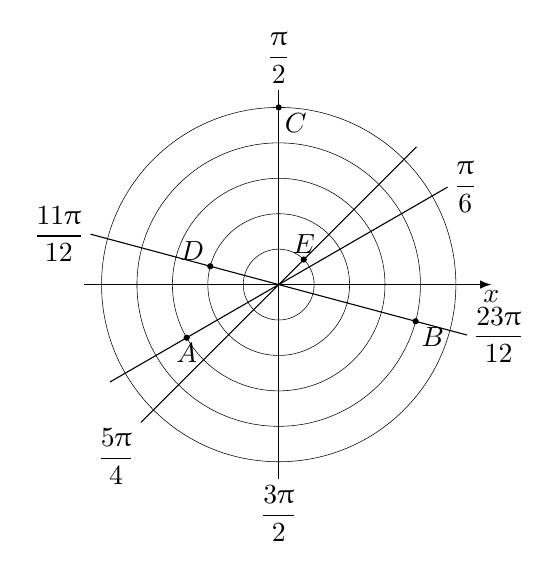
\begin{tikzpicture}[>=latex,scale=0.45,inner sep=2pt]
  \draw[thin,->](-5.5,0)--(6,0)node[below]{$x$};
  \foreach \x/\t/\p in {30/{\dfrac{\uppi}{6}}/right,90/{\dfrac{\uppi}{2}}/above,165/{\dfrac{11\uppi}{12}}/left,225/{\dfrac{5\uppi}{4}}/below left} 
    { 
      \draw(\x:-5.5)--(\x:5.5);
      \node at (\x:5.5)[\p]{$\t$}; 
    }
  \node at (-90:5.5)[below]{$\dfrac{3\uppi}{2}$};
  \node at (-15:5.5)[right]{$\dfrac{23\uppi}{12}$};
  \foreach \x/\t/\p[count=\i]  in {45/E/above,165/D/above left,210/A/below,-15/B/below right,90/C/below right}
  {
    \draw[very thin](0,0)circle(\i);
    \fill (\x:\i)circle(2.5pt)node[\p]{$\t$}; 
  }
\end{tikzpicture}
\end{document}